\message{ !name(s4.tex)}\documentclass[11pt]{article}
%Gummi|063|=)
\title{\textbf{Algorithms I -- supervision 5}}
\author{James Wood}
\usepackage{listings}
\usepackage{bold-extra}
\usepackage{xcolor}
\usepackage{amsmath}
\usepackage{enumitem}
\usepackage{tikz}
\usetikzlibrary{arrows}

\lstset{
  basicstyle=\small,
  basewidth=0.5em,
  frame=single,
  breaklines=true,
  %postbreak=\raisebox{0ex}[0ex][0ex]{
  %  \ensuremath{\color{red}\hookrightarrow\space}
  %}
  language=python,
  literate=
    {<=}{{\(\leq\)}}1
    {>=}{{\(\geq\)}}1
    {&&}{{\(\wedge\)}}1
    {||}{{\(\vee\)}}1
    {->}{{\(\rightarrow\)}}1
}

\tikzset{
  treenode/.style = {align=center, inner sep=0pt, text centered,
    font=\sffamily},
  bnode/.style = {treenode, circle, white, draw=black,
    fill=black, text width=1.5em},
  rnode/.style = {treenode, circle, red, draw=red,
    text width=1.5em, very thick},
  leaf/.style = {treenode, rectangle, draw=black,
    minimum width=0.5em, minimum height=0.5em}
}

\begin{document}

\message{ !name(s4.tex) !offset(141) }
 (black) nodes.
\item
  A rotation about a node of a binary search tree is an operation that moves one of the children of the node into its parent's place, moving the parent into the subtree opposite to the one the child came from. Then, the three subtrees of these two nodes are reättached in order. Consider this example:

  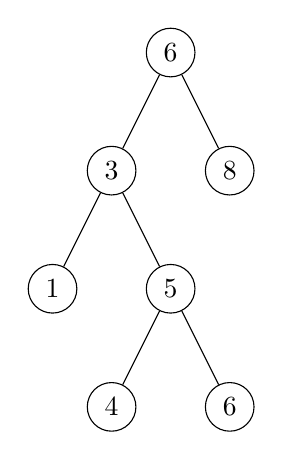
\begin{tikzpicture}
    \node[circle,draw](z){6}
    child{
      node[circle,draw]{3}
      child{node[circle,draw]{1}}
      child{
        node[circle,draw]{5}
        child{node[circle,draw]{4}}
        child{node[circle,draw]{6}}
      }
    }
    child{
      node[circle,draw]{8}
    };
  \end{tikzpicture}

  To perform a leftward rotation on the 3 node, the 5 node is moved in place of the 3 node, and the 3 node and its left subtree are reättached under the 5 node. Then, the 4 subtree is moved to become the other subtree of the 3 node, and the 6 subtree becomes the right subtree of the 5 node again. This yields:

  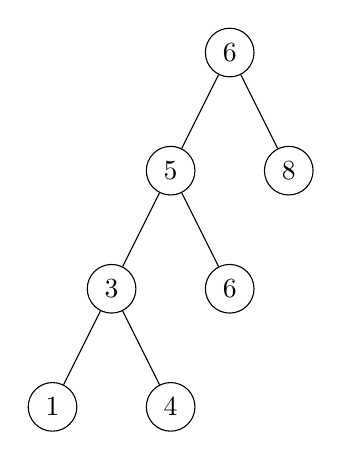
\begin{tikzpicture}
    \node[circle,draw](z){6}
    child{
      node[circle,draw]{5}
      child{
        node[circle,draw]{3}
        child{node[circle,draw]{1}}
        child{node[circle,draw]{4}}
      }
      child{node[circle,draw]{6}}
    }
    child{
      node[circle,draw]{8}
    };
  \end{tikzpicture}
\item To transform BST 
\message{ !name(s4.tex) !offset(281) }

\end{document}